\documentclass[12pt]{article}
% add some essential packages, some might not be used

\usepackage[T1]{fontenc}
\usepackage[utf8]{inputenc}
\usepackage[usenames,dvipsnames]{color}
\usepackage{natbib}
\usepackage{authblk}
\usepackage{ragged2e}
\usepackage{amsmath}
\usepackage[a4paper,margin=1in,bottom=1.0in]{geometry}
\usepackage{url}
\usepackage{array}
\usepackage{bbding}
\usepackage{amssymb}
\usepackage{graphicx}  % mini page function
\usepackage{adjustbox}
\usepackage{subcaption}
\usepackage{booktabs}
\usepackage{float}
\usepackage{appendix} % appendix package
\usepackage{hyperref}
\usepackage{url}
\usepackage[english]{babel}
\usepackage{adjustbox}
\usepackage{enumitem}
\usepackage{textgreek}
\usepackage{bibentry}
\nobibliography*
\usepackage{lipsum}


\usepackage{listings}
\usepackage{wasysym}
\usepackage{amsthm}
\usepackage{framed}
\usepackage{bm}
\usepackage{booktabs}  % package for table line
% \usepackage{amsrefs?}  % ams citation style package


\usepackage{rotating} % for the horizontal page table

\usepackage{tikz}
\usetikzlibrary{calc}
\usetikzlibrary{matrix}
\usetikzlibrary{positioning}
\usepackage{color}
\usepackage{setspace}
\usepackage{xcolor}

\usepackage{tcolorbox} % package for making colorful box

 \setlength{\parskip}{0.15cm} % change the paragraph spacing
\renewcommand\labelitemi{$\vcenter{\hbox{\tiny$\bullet$}}$} % set the bullet size as tiny

% \newcommand*\rot{\rotatebox{90}} % for rotate text

\usepackage{sectsty} %package for section size

\sectionfont{\fontsize{14}{12}\selectfont} % Change the section font size

\subsectionfont{\fontsize{13}{12}\selectfont}
\subsubsectionfont{\fontsize{12}{12}\selectfont}

\newcommand\numberthis{\addtocounter{equation}{1}\tag{\theequation}} % new command



\theoremstyle{definition}
\newtheorem{definition}[subsection]{Definition}
\newtheorem{axiom}[subsection]{Axiom}
\newtheorem{example}[subsubsection]{Example}
\newtheorem{theorem}[subsection]{Theorem}
\newtheorem{proposition}[subsection]{Proposition}
\newtheorem{lemma}[subsection]{Lemma}


\usepackage{courier}

% tikzsetting

\usetikzlibrary{shapes,decorations,arrows,calc,arrows.meta,fit,positioning}

\tikzset{
    -Latex,auto,node distance =1 cm and 1 cm,semithick,
    state/.style ={ellipse, draw, minimum width = 0.7 cm},
    point/.style = {circle, draw, inner sep=0.04cm,fill,node contents={}},
    bidirected/.style={Latex-Latex,dashed},
    el/.style = {inner sep=2pt, align=left, sloped}
}

\lstset{language=R}

\definecolor{mygreen}{rgb}{0,0.6,0}
\definecolor{mygray}{RGB}{145, 153, 165}
\definecolor{mymauve}{rgb}{0.58,0,0.82}

\lstset{
  backgroundcolor=\color{white},   % choose the background color; you must add \usepackage{color} or \usepackage{xcolor}; should come as last argument
  basicstyle=\footnotesize,        % the size of the fonts that are used for the code
  breakatwhitespace=false,         % sets if automatic breaks should only happen at whitespace
  breaklines=true,                 % sets automatic line breaking
  captionpos=b,                    % sets the caption-position to bottom
  commentstyle=\color{gray},    % comment style
  deletekeywords={...},            % if you want to delete keywords from the given language
  escapeinside={\%*}{*)},          % if you want to add LaTeX within your code
  extendedchars=true,              % lets you use non-ASCII characters; for 8-bits encodings only, does not work with UTF-8
  frame=single,	                   % adds a frame around the code
  keepspaces=true,                 % keeps spaces in text, useful for keeping indentation of code (possibly needs columns=flexible)
  keywordstyle=\color{RoyalBlue},       % keyword style
  language=R,                 % the language of the code
  morekeywords={*,...},            % if you want to add more keywords to the set
  numbers=left,                    % where to put the line-numbers; possible values are (none, left, right)
  numbersep=5pt,                   % how far the line-numbers are from the code
  numberstyle=\tiny\color{gray}, % the style that is used for the line-numbers
  rulecolor=\color{black},         % if not set, the frame-color may be changed on line-breaks within not-black text (e.g. comments (green here))
  showspaces=false,                % show spaces everywhere adding particular underscores; it overrides 'showstringspaces'
  showstringspaces=false,          % underline spaces within strings only
  showtabs=false,                  % show tabs within strings adding particular underscores
  stepnumber=2,                    % the step between two line-numbers. If it's 1, each line will be numbered
  stringstyle=\color{mymauve},     % string literal style
  tabsize=2,	                   % sets default tabsize to 2 spaces
  title=\lstname                   % show the filename of files included with \lstinputlisting; also try caption instead of title
}

\numberwithin{equation}{section}
\numberwithin{figure}{section}
\numberwithin{table}{section}


% Define colors
\definecolor{cmd}{HTML}{F7F7F9}
\DeclareMathOperator{\di}{d\!}

\newcommand{\pr}{$\mathbb{P}$}
\newcommand{\pre}{\mathbb{P}}

\begin{document}

\title{Investment and Financial Risk}
\author{Michael}
\date{}
\maketitle

\begin{abstract}
  In non-stational time series part, I have checked the main US economic time series of interested: real GDP, real investment, real consumption, Dow Jones Industrial Average,
NASDAQ Composite Index, S\&P 500 Index. The unit root tests showed that all those time series follows the random walk with drift process, or $I(1)$. By simply plotting those time series, I found a very interesting patter, which implies that investment is very special. It's growth rate can be modeled with univariate volatility modeling. This notes will study the relationship between investment and financial risk.
\end{abstract}


\section{Review of Non-stationary Time Series}

First, let's review the non-stationary time series by analysing the following equation again,
\begin{figure}[H]
  \centering
  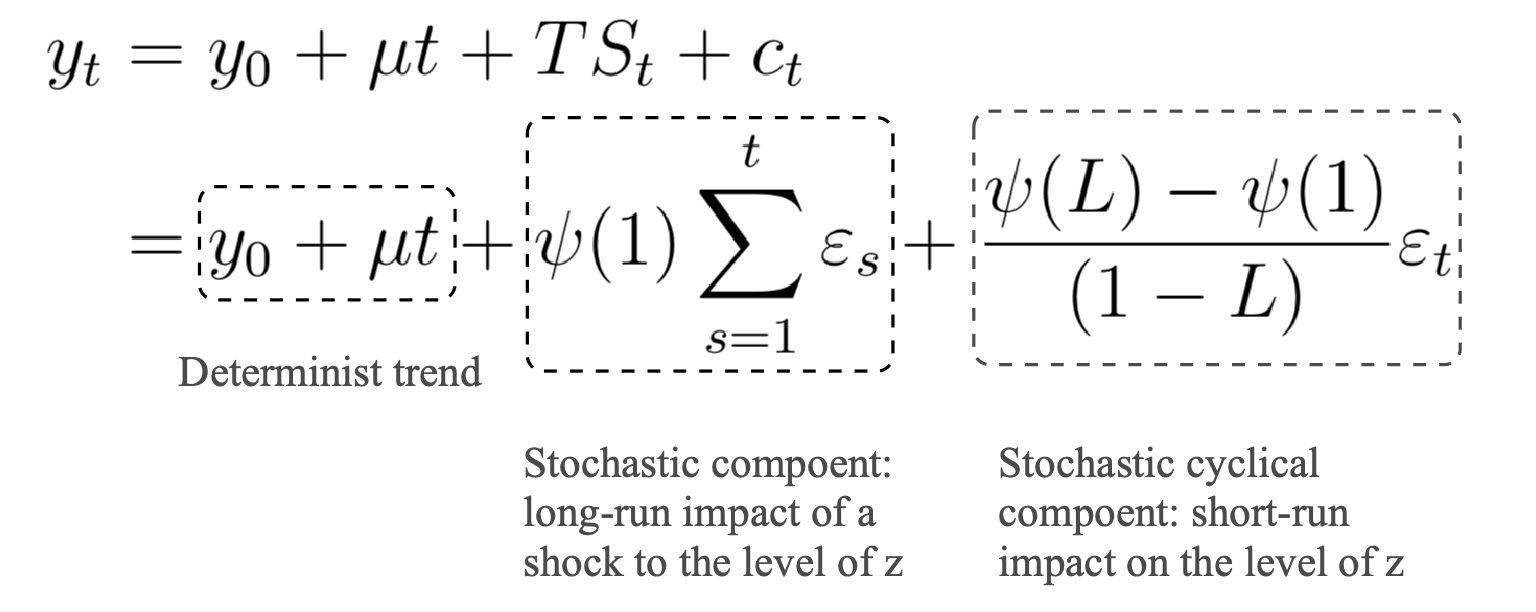
\includegraphics[width=0.69\textwidth]{ydecom}
  \caption{Intuition on $y_t$ decomposition}
\end{figure}

From the figure 1.1, we can state that if the time series follows the unit root with drift, it can be modeled with the following equation:
\begin{align}
  y_t  &  = y_0 + TS_t + c_t \\
  & = y_0 + \psi(1) \sum_{s=1}^t \varepsilon_s + \frac{\psi(L) - \psi(1)}{(1- L)} \varepsilon_t
\end{align}

This means that the economic growth is the result of sum of technology shocks. Intuitively, I believe it is true. Look at China, people are same right now and 30 years ago. Many scholars argued that the miracle of China economy is due to the cheap labor with considering the labor in North Korea is even much cheaper than China. Again, people are the same before the rapid growth of economy. They were not either super smart or super stupid. They have just learned how to manufacture goods rapidly with the foreign direct investment. In the end, I believe that economic growth is just the revealing process of technology through investment (including investment on education).

Some people might argue that innovation is an endogenous factor of economic growth by giving America as a convincing example. Yes, I agree with this. But, I have to restate that it is still the revealing process of technology or truth. Man does not create science, man only discovers science. If we can do an imaginary experiment that let anyone who are interested on science do their work generations by generations, I believe that the scientific discovery will follows some distributions(let's say, normal distribution\footnote{If you are familiar with the derivation of normal distribution, which is the reflection of error generating process, you will not doubt me.}) across different countries. The reason that some coutries, like USA, UK, Germany, France, etc., can have more innovations is that they allocate more resources on science. Yes, any country can \textit{reveal or discovery} science as long as people there are doing it in scientific ways. According to Acemoglu, it's all about institutions.

\section{Review of Joseph Schumpeter}

Once we reached the conclusion that economic growth is the revealing process of technology or truth through the investment, we need review the study by the great economist - \textit{Joseph Schumpeter\footnote{Reading this guy you will realise that math is not the only thing matters for economists.}}. Like the paper by \cite{aghion1990model}, I will just quote from the book by \cite{schumpeter2010capitalism}:
\begin{quotation}
 The fundamental impulse that sets and keeps the capitalist engine in motion comes from the new consumers' goods, the new methods of production or transportation, the new markets,...[This process] is incessantly revolutionises the economic structure form within, incessantly destroying the old one, incessantly creating a new one. This process of Creative Destruction is the essential fact about capitalism.
\end{quotation}

Although paper by \cite{romer1990endogenous} and \cite{aghion1990model} have extensively analysed the endogenous growth pattern, they still missed the capitalism part, especially on the capitalism with asymmetric information\footnote{I will analyse the investment with asymmetric information in next notes.}. In 1911, \citeauthor{schumpeter2017theory} argued that the services provided by financial intermediaries-mobilizing savings, evaluating projects, managing risk, monitoring managers, and facilitating transactions-are essential for technological innovation and economic development.

I am a man who always observe the real world, the picture described by Schumpeter is so common in our real life. Investment is full of risk, if risk and expectation on future profits are not clear, no one is willing to get involved in this kind of game. The gamblers (or so called risk-lover) are shaped by the expectations. The hesitaters are shaped by the risk.

In conclusion, without risk-based pricing and investment through financial markets, capitalism cannot expand in a large scale. Even individuals or individual firms invest projects by themselves, evaluation on risk and future profit is still very essential. This implies economic growth models without risky investment are defective or faulty.

\section{Investment and Financial Risk}

Before modeling investment with univariate volatility modeling, let's check the plots first.
\begin{figure}[H]
  \centering
  \begin{subfigure}[b]{0.85\textwidth}
    \centering
    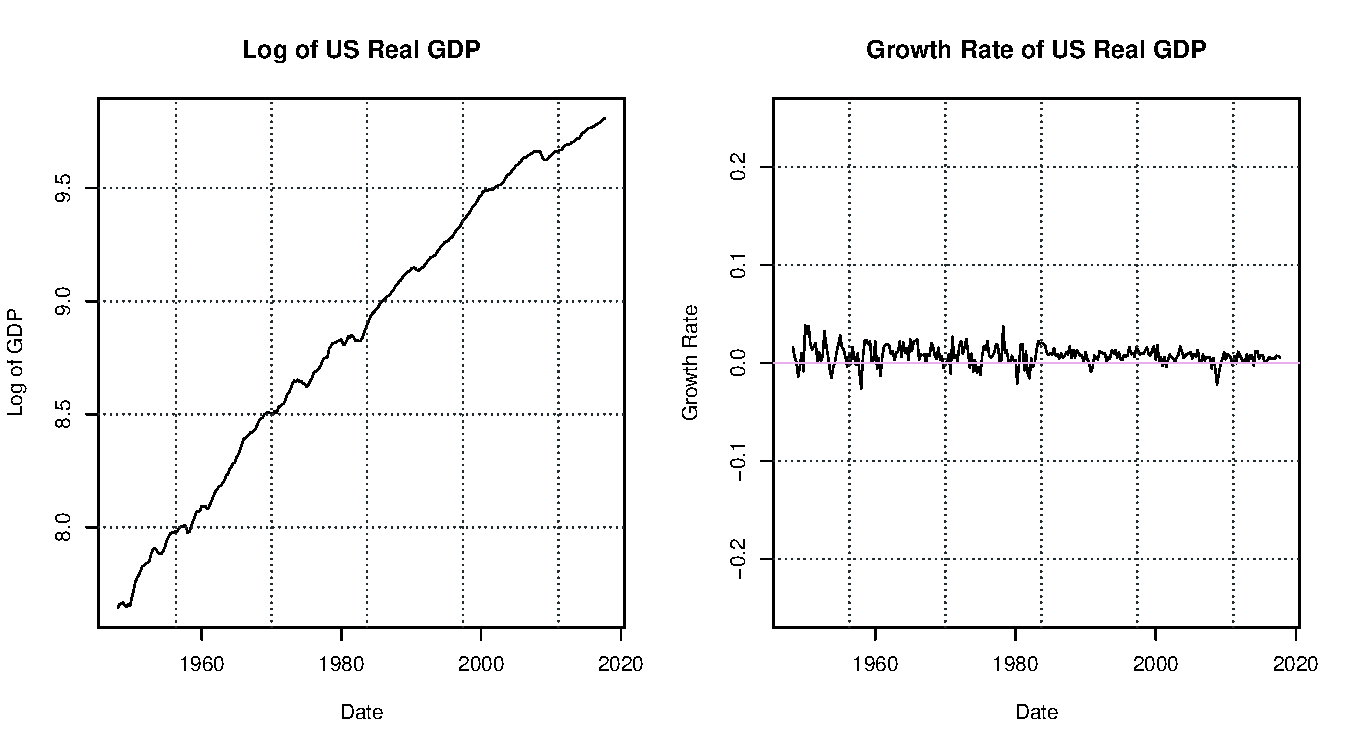
\includegraphics[width=\textwidth]{../Figures/usrealgdp}
  \end{subfigure}
  \begin{subfigure}[b]{0.85\textwidth}
    \centering
    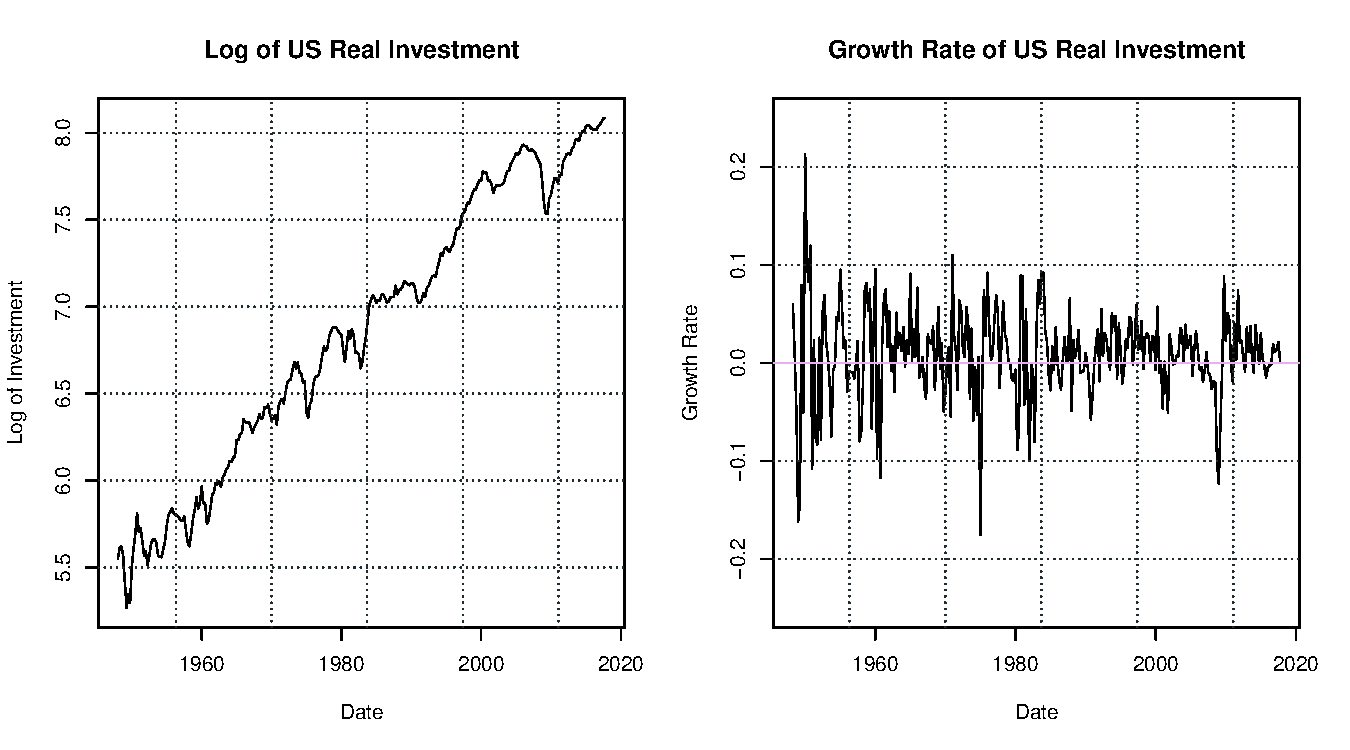
\includegraphics[width=\textwidth]{../Figures/usInv}
  \end{subfigure}
  \begin{subfigure}[b]{0.85\textwidth}
    \centering
    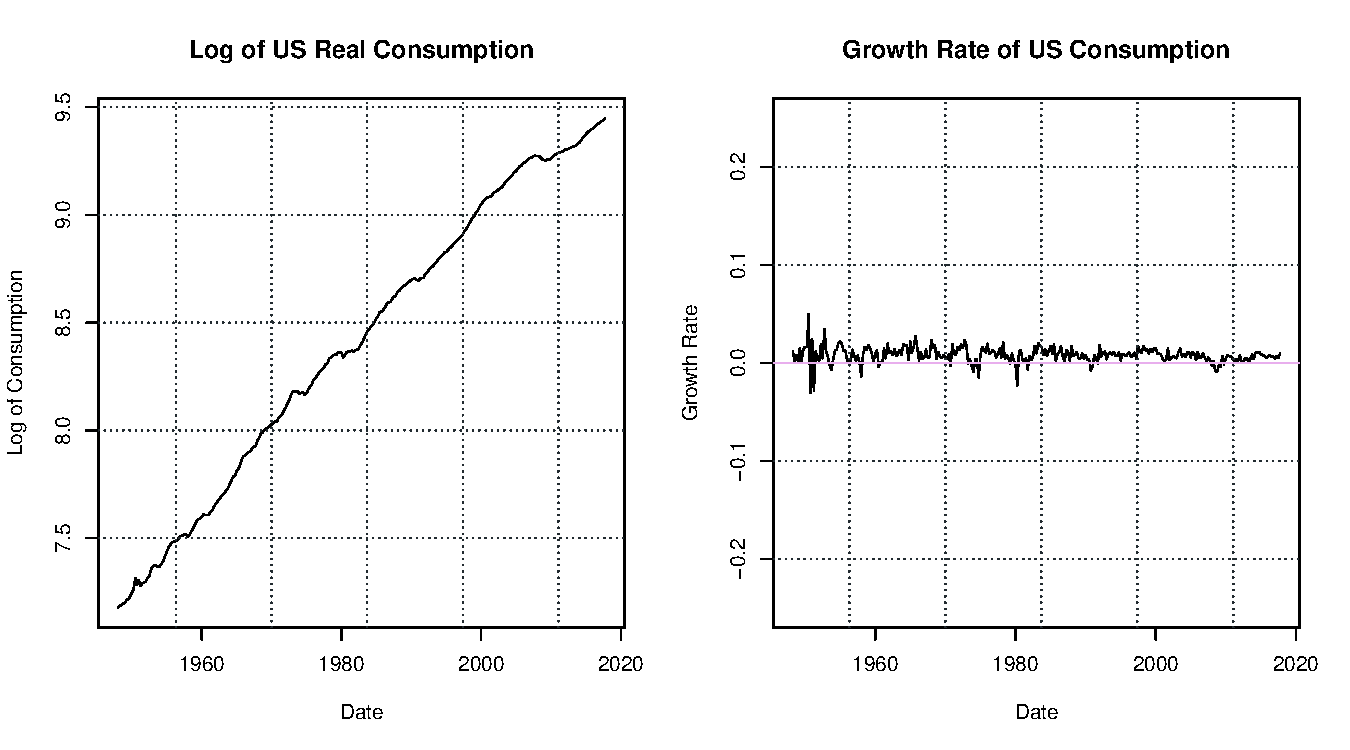
\includegraphics[width=\textwidth]{../Figures/usCons}
  \end{subfigure}
\end{figure}

It's very easy to spot that US real investment has higher volatility compared to real GDP and consumption. Now, if we put investment and financial market index plots together, the pattern is more clear.
\begin{figure}[H]
  \centering
  \begin{subfigure}[b]{0.85\textwidth}
    \centering
    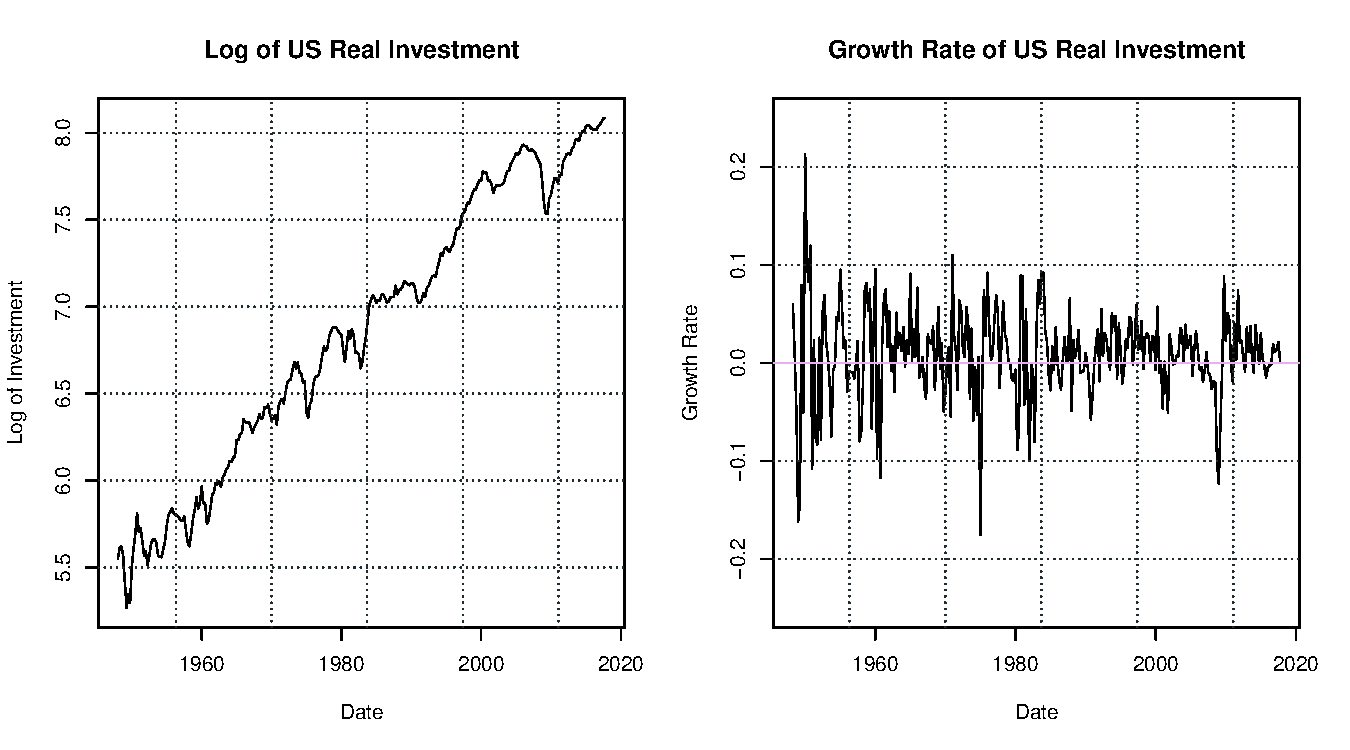
\includegraphics[width=\textwidth]{../Figures/usInv}
  \end{subfigure}
  \begin{subfigure}[b]{0.85\textwidth}
    \centering
    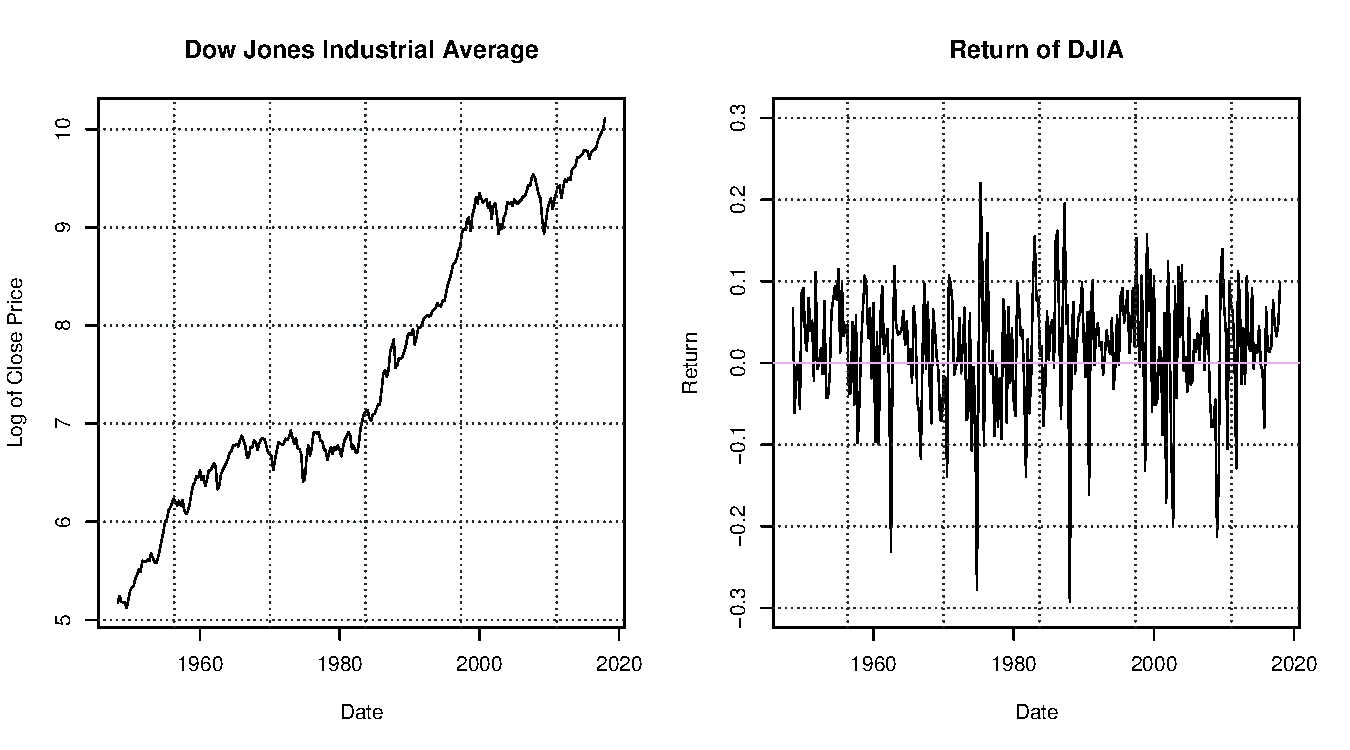
\includegraphics[width=\textwidth]{../Figures/usDJIA}
  \end{subfigure}
  \begin{subfigure}[b]{0.85\textwidth}
    \centering
    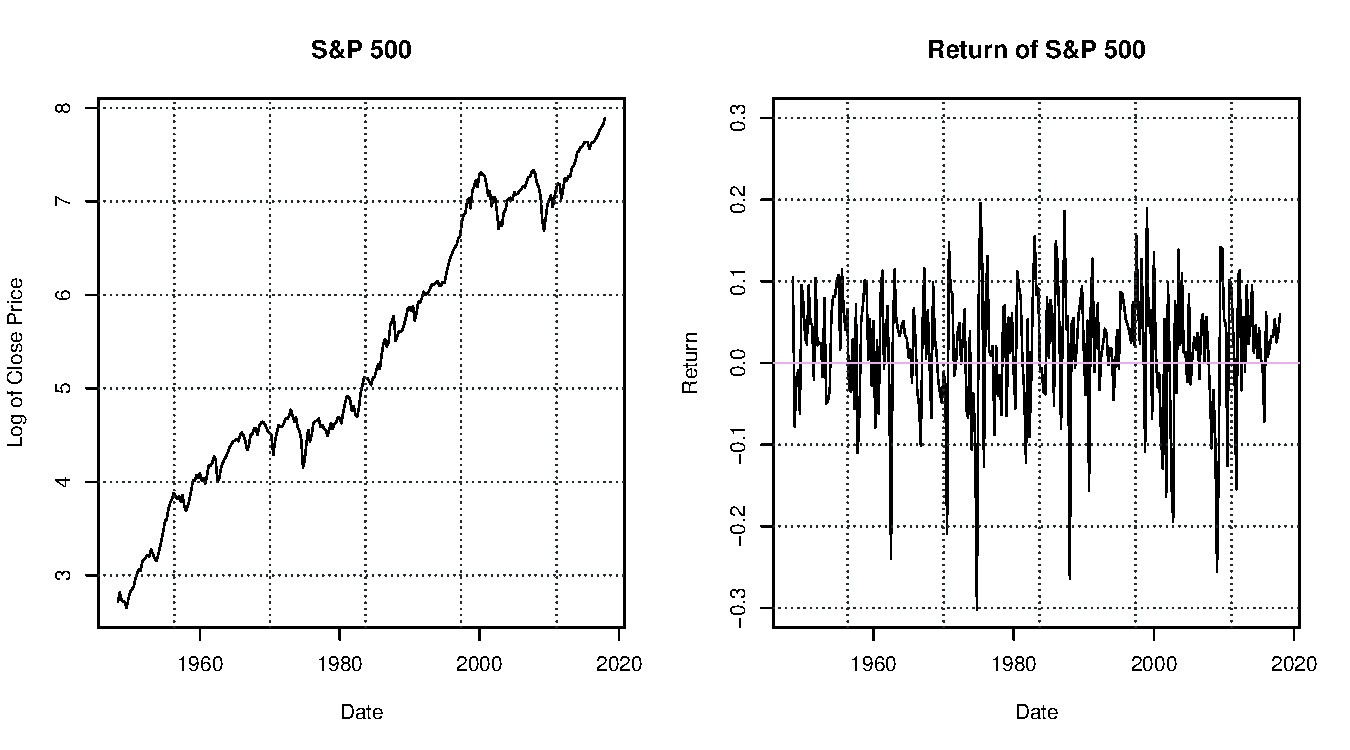
\includegraphics[width=\textwidth]{../Figures/usSPX}
  \end{subfigure}
\end{figure}

\section{The Stylized Facts of Investment}

Compare the volatility of real investment with SP500, we can see that real investment also has the volatility clusters. It should not be surprised that the volatility of real investment is lower than SP500 considering the investment activities in stock market is more intense.
\begin{figure}[H]
  \centering
  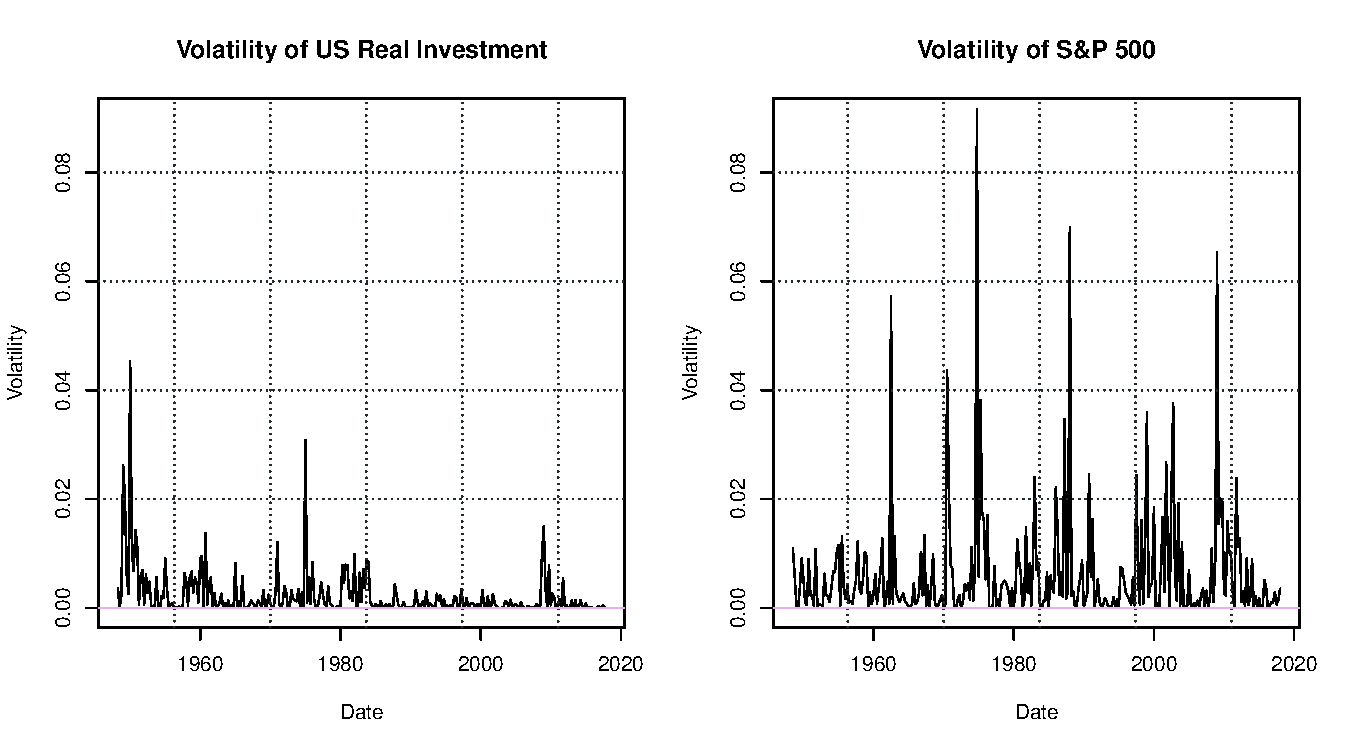
\includegraphics[width=\textwidth]{../Figures/VolatInvSP500}
\end{figure}
It's very interesting that the autocorrelation for real investment volatility remains longer than that of SP500 based on the next figure. Since we are using quarterly time series, the volatility pattern of SP500 almost die out in such a long time window.
\begin{figure}[H]
  \centering
  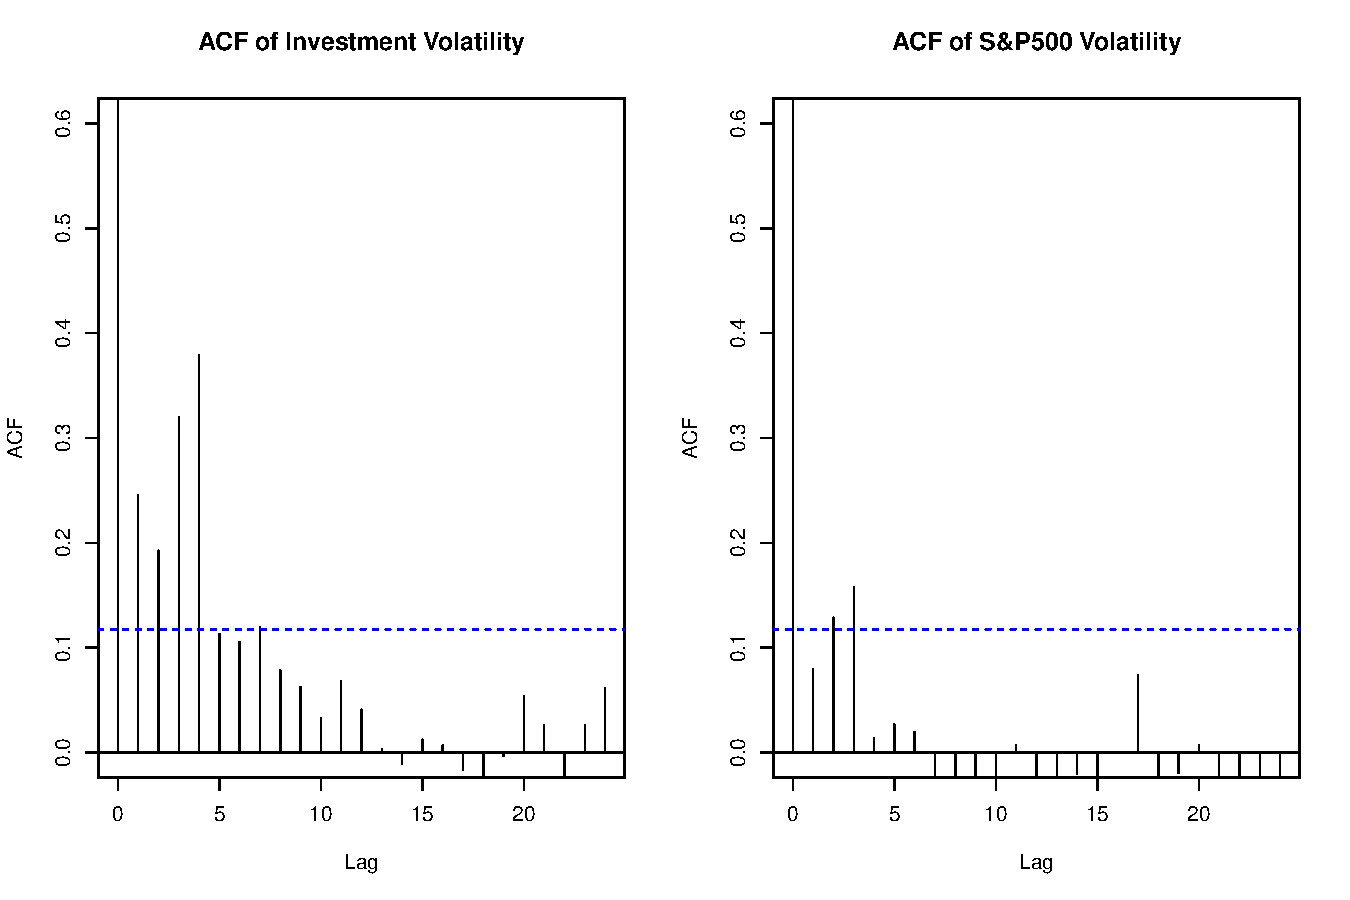
\includegraphics[width=0.9\textwidth]{../Figures/AcfInvSP500}
\end{figure}

Considering the there is significant autocorrelation for the volatility of investment, we model it with the following GARCH model first
\begin{align}
  I_t = \sigma_t \varepsilon_t; \ \ \ \sigma_t^2 = \omega + \alpha I_{t-1}^2
\end{align}
Table 4.1 gives the estimation results based on the normal distribution.
\begin{table}[H]
  \centering
  \renewcommand{\arraystretch}{1.2}
  \caption{ARCH estimation for volatility of Investment}
\begin{tabular}{lccccc}
  \hline
         & Estimate & Std. Error & t value & Pr(\textgreater{}|t|)  \\
         \hline
 $\omega$    &14.3605      &1.6711   & 8.593 & \textless 2e-16 & ***   \\
$\alpha$    & 0.3690   &    0.1102    & 3.347 & 0.000817 & ***  \\
 \hline
\end{tabular}
\end{table}

If we fit the GARCH model, we should fit
\begin{align}
  I_t = \sigma_t \varepsilon_t; \ \ \ \sigma_t^2 = \omega + \alpha I_{t-1}^2 + \beta \sigma_{t-1}^2
\end{align}
\begin{table}[H]
  \centering
  \renewcommand{\arraystretch}{1.2}
  \caption{GARCH estimation for volatility of Investment}
\begin{tabular}{lccccc}
  \hline
         & Estimate &  Std. Error & t value & Pr(\textgreater{}|t|) \\
         \hline
$\omega$& 0.0001949 &  0.0001046  &  1.864 & 0.06239 &. \\
 $\alpha$ & 0.1970969 &  0.0663127  &  2.972 & 0.00296& ** \\
 $\beta$ & 0.7128599 &  0.0926045 &   7.698 &1.38e-14& *** \\
 \hline
\end{tabular}
\end{table}

If we fit the model based on (4.2) with student-t distribution, we get the following results.
\begin{table}[H]
  \centering
  \renewcommand{\arraystretch}{1.2}
  \caption{GARCH estimation for volatility of Investment (Student-t)}
\begin{tabular}{lccccc}
  \hline
         & Estimate &  Std. Error & t value & Pr(\textgreater{}|t|) \\
         \hline
 $\omega$& 0.000145  & 9.345e-05  &  1.548 & 0.12150 \\
$\alpha$&0.2309  & 0.08157&  2.830 & 0.00465 &** \\
$\beta$& 0.7195 & 0.08704  &  8.267 &2.22e-16 &*** \\
shape &  6.148 &  2.139 &    2.874 & 0.00405 & ** \\
\hline
\end{tabular}
\end{table}

Considering all coefficients are significant, we have to provide the interpretations behind this GARCH model. Again, let's start it from the equation
\begin{align}
  I_t = \sigma_t \varepsilon_t; \ \ \ \sigma_t^2 = \omega + \alpha I_{t-1}^2 + \beta \sigma_{t-1}^2,
\end{align}
where $I_t$ is the investment growth rate, or investment innovation at time $t$. It is derived by de-mean the data:
\begin{align}
  I_t = Y_t - E[Y_t | \mathcal{F}_{t-1}]
\end{align}
The investment shock or investment innovation will affect the investment growth rate $Y_t$ based one (4.4). Although we don’t know $I_t$, we can further assume it can be represented by $\sigma_t$ and $\varepsilon_t$, where $\varepsilon_t \sim i.i.d(0, 1)$. That's why we have
\begin{align}
  I_t = \sigma_t \varepsilon_t
\end{align}

What's the economic interpretation of $\sigma_t$ and $\varepsilon_t$? We know that $\sigma_t$ is the conditional volatility and $\varepsilon_t$ is the exogenous shocks. Now, let's write the full model
\begin{align}
  Y_t & = E[Y_t | \mathcal{F}_{t-1}] + I_t \\
  I_t & = \sigma_t \varepsilon_t \\
  \sigma_t^2 & = \omega + \alpha I_{t-1}^2 + \beta \sigma_{t-1}^2
\end{align}

In words, the investment growth rate $Y_t$ depends on the conditional mean and investment innovation shocks. Intuitively, this is aligned with our common sense where anyone will investment based on the past trend (conditional mean) and technology innovations. The technology innovations then can be decomposed into two parts: conditional volatility $\sigma_t$ and exogenous technology shocks $\varepsilon_t$. This is also aligned with our common sense that we invest based on the conditional volatility\footnote{Think about the BigData investment fever, people buy and sell similar projects and stocks very often.} and exogenous technology shocks. In the end, the conditional volatility evolves with the previous innovations and itself.

In conclusion, the investment is driven by two factors: financial risk (conditional volatility) and exogenous technology shocks. Meanwhile, financial risk (conditional volatility) also involves with exogenous technology shocks. The whole mechanism behind (4.6) to (4.8) can be understood as a technology revealing process with the buffer.

Assume positive and negative technology shocks $\varepsilon_t$ have the same effects for the moment, people will only continue increase the investment condition on the cases that profound technology shocks keep come incessantly\footnote{That's the beautify of autoregressive conditional heteroskedasticity model.}.















\newpage
\bibliography{/Users/Michael/Documents/DSGE/dsge.bib}
\bibliographystyle{apalike}
\end{document}
